% SPDX-License-Identifier: MIT
% Part of lgpsf — https://github.com/NickAlger/lgpsf
%
% The heat-inversion tutorial: the complete lgpsf pipeline on one small
% PDE inverse problem. Every figure is produced, and every code snippet
% extracted, by make_figures.py in this directory — the committed PDF is
% built from the exact code that made its figures.
%
% Build: pdflatex heat-pipeline.tex  (twice, for references)
\documentclass[11pt]{article}

\usepackage[margin=1.1in]{geometry}
\usepackage{amsmath, amssymb}
\usepackage{graphicx}
\usepackage[colorlinks=true, linkcolor=blue, urlcolor=blue]{hyperref}

\newcommand{\Hd}{H_d}
\newcommand{\Hr}{H_r}

\title{LGPSF Heat Inverse Problem Tutorial}
\author{}
\date{}

\begin{document}
\maketitle
\vspace{-3em}

\begin{abstract}
\noindent
This tutorial walks the complete lgpsf pipeline through one small but
genuine PDE inverse problem, start to finish: pose the problem, look at
the Hessian's point-spread functions, fit them from a handful of matrix
probes, certify and correct the fit, choose the regularization parameter
with the fitted operator doing the preconditioning, and watch what the
preconditioner does to the spectrum and to the reconstruction dynamics.
Every figure is produced by \texttt{make\_figures.py} in this directory,
and every code snippet is extracted from that file rather than
transcribed, so this document is built from the exact code that made its
figures.
\end{abstract}

\section{The inverse problem}

Heat diffuses through the unit square for a short time $T$; we observe
the result everywhere, once, and want the initial condition back. The
thermal conductivity $\kappa$ is piecewise constant with sharp jumps
(Figure~\ref{fig:problem}, center): a conductive slab on the left
($\kappa = 1$), an insulating pocket on the lower right
($\kappa = 0.005$), and background between ($\kappa = 0.1$) --- a
$200\times$ contrast. On a $32 \times 32$ cell-centered grid
($n = 1024$, spacing $h$), the forward map is implicit Euler with eight
steps,
\[
  A \;=\; \bigl(I + \tfrac{T}{8} L_\kappa\bigr)^{-8},
  \qquad
  L_\kappa = -\nabla\!\cdot\!(\kappa \nabla \cdot)
  \ \text{(harmonic face averages, zero Dirichlet)},
\]
with $T = 0.01$. Given noisy data $d = A u_0 + \eta$, Tikhonov
regularization minimizes
\[
  J(u_0) \;=\; \tfrac{1}{2}\, h^2 \|A u_0 - d\|^2
  \;+\; \tfrac{a}{2}\, u_0^T \Hr\, u_0 ,
  \qquad\text{i.e.}\qquad
  (\Hd + a \Hr)\, u_0 \;=\; h^2 A^T d,
\]
where $\Hd = h^2 A^T A$ is the data-misfit Hessian and $\Hr$ is the
$H^1$-seminorm stiffness matrix (the $\kappa$-free Laplacian). One
application of $\Hd$ costs two PDE solves. That cost is the whole
subject of this tutorial: everything below is about never forming
$\Hd$, and about spending as few applications of it as possible.

The true initial condition carries features at two scales --- one broad
blob and four sharp spots --- placed deliberately in each material
region:

{\small\begin{verbatim}
# The true initial condition carries features at TWO scales: one broad
# blob spanning the conductive slab's boundary, and four sharp spots --
# in the pocket, the background, and the slab. The scale separation is
# what the final figure of the paper is built to expose.
def gaussian(center, width, amplitude=1.0):
    d2 = ((x[0] - center[0]) ** 2 + (x[1] - center[1]) ** 2)
    return amplitude * np.exp(-0.5 * d2 / width**2)

u0 = (gaussian((0.42, 0.62), 0.16)
      + 0.9 * gaussian((0.75, 0.30), 0.02)     # in the insulating pocket
      + 0.8 * gaussian((0.70, 0.75), 0.02)     # in the background
      - 0.7 * gaussian((0.22, 0.35), 0.02)     # in the slab, signed
      + 0.8 * gaussian((0.15, 0.80), 0.02))    # in the slab
\end{verbatim}
}

\noindent
The data is the diffused field plus $1.5\%$ iid noise:

{\small\begin{verbatim}
# Observe the diffused field everywhere at the final time, with iid
# noise at 1.5% of the signal's RMS -- the data a real inversion holds.
rng = np.random.default_rng(SEED)
observed = problem["propagate"](u0)                        # A u0
noise = NOISE * np.sqrt(np.mean(observed**2))
data = observed + noise * rng.standard_normal(observed.shape)
\end{verbatim}
}

\begin{figure}[htb]
  \centering
  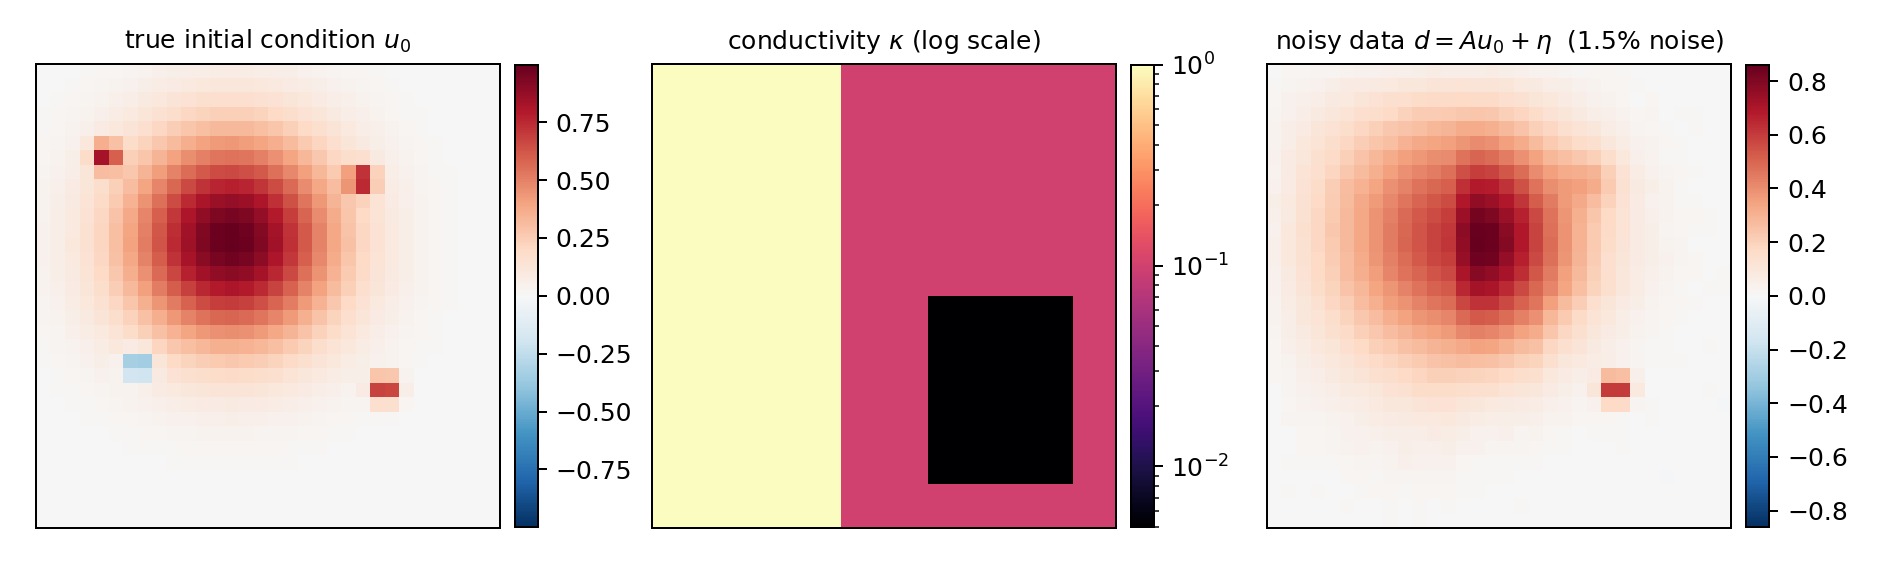
\includegraphics[width=\textwidth]{figures/problem.png}
  \caption{\textbf{(The problem.)} Left: the true initial condition
    $u_0$, a broad blob plus four sharp spots. Center: the conductivity
    $\kappa$ on a log color scale; the jumps are the story. Right: the
    noisy data $d = A u_0 + \eta$. The data already foretells the
    reconstruction results of Section~\ref{sec:lcurve}: the spot in the
    insulating pocket survives diffusion nearly intact, while the spots
    in the conductive slab are smeared beyond recovery.}
  \label{fig:problem}
\end{figure}

\section{The Hessian's rows are local, but not Gaussian}

Row $i$ of $\Hd$ is the point-spread function (PSF) of ``diffuse for
time $2T$,'' anchored at grid point $x_i$: a bump whose width scales
like $\sqrt{T\kappa}$ and whose magnitude varies with $\kappa$, so the
row norms span more than two orders of magnitude across the domain.
Sampling one row costs one application of $\Hd$:

{\small\begin{verbatim}
# A row of the Hessian is the point-spread function of "diffuse for
# time 2T", anchored at that row's grid point. Sampling one costs two
# PDE solves -- H_d e_i by the matrix-free apply.
def psf(index):
    impulse = np.zeros(problem["count"])
    impulse[index] = 1.0
    return problem["apply_Hd"](impulse)
\end{verbatim}
}

Figure~\ref{fig:psfs} shows six sampled rows. Away from the jumps the
PSFs are clean isotropic near-Gaussians --- broad and shallow in the
slab, narrow in the background, nearly a point in the pocket. The
interesting rows sit \emph{on} the jumps: heat floods into the
conductive side and stalls at the insulating one, so an interface PSF is
skewed and two-sided. These are the rows a spatially-varying Gaussian
model cannot represent, and the reason lgpsf carries higher
Laguerre--Gaussian modes.

\begin{figure}[htb]
  \centering
  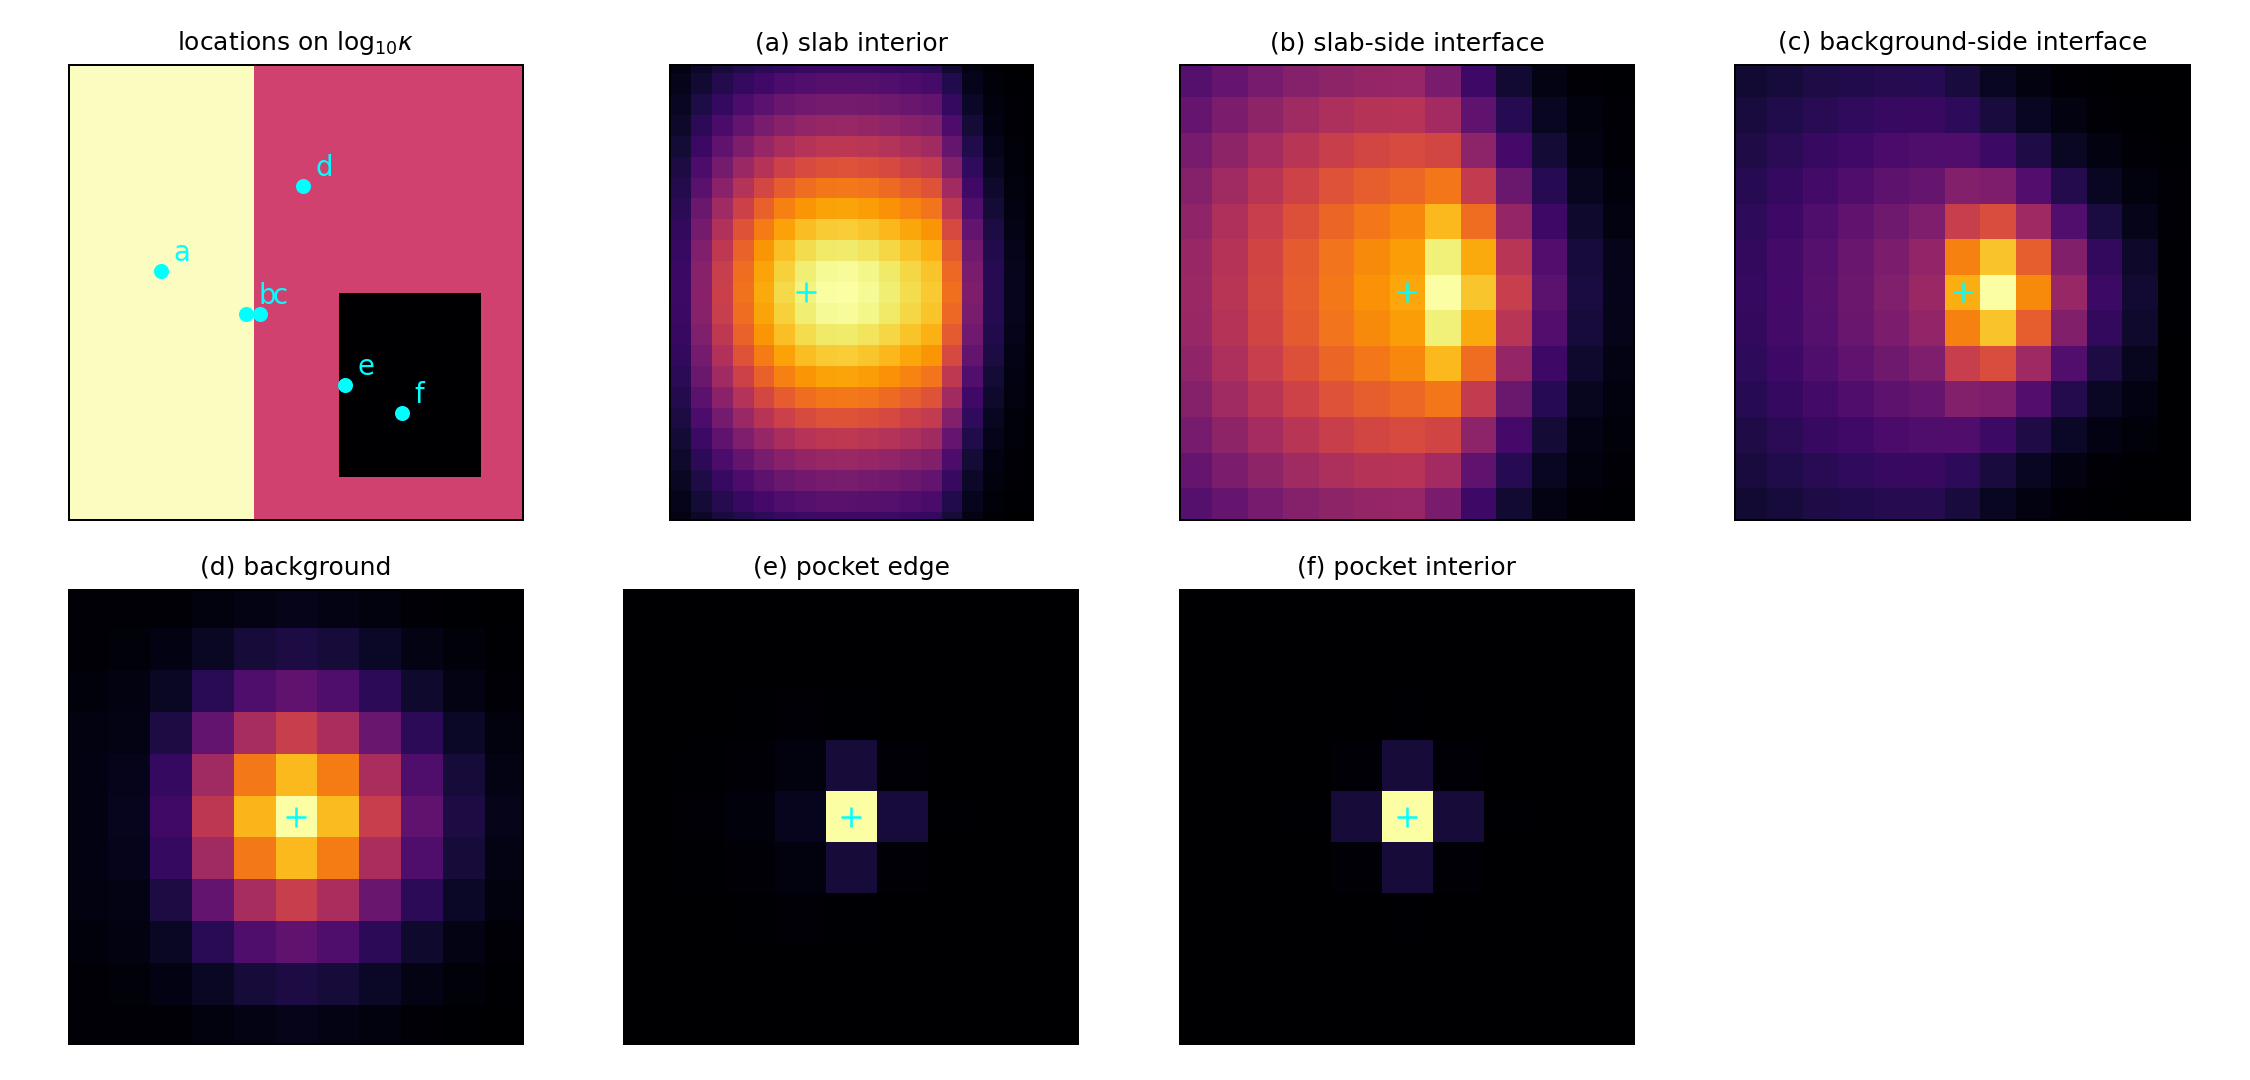
\includegraphics[width=\textwidth]{figures/psfs.png}
  \caption{\textbf{(Sampled impulse responses.)} Six rows of $\Hd$,
    each panel zoomed to its own neighborhood; cyan markers on the
    $\log_{10}\kappa$ panel give the anchor locations, and the cyan
    ``$+$'' marks each anchor. (a)~slab interior: broad and shallow.
    (b)~slab-side interface: mass fills the slab and piles up in a
    ridge against the jump. (c)~background-side interface: a compact
    peak whose tail leaks into the slab. (d)~background: a clean
    near-Gaussian. (e), (f)~pocket: nearly point masses. Local
    everywhere --- Gaussian only away from the jumps.}
  \label{fig:psfs}
\end{figure}

\section{Fitting the operator from a handful of probes}

The fitter never sees $\Hd$'s entries. It sees $k$ random probes and
their responses --- $k$ applications of $\Hd$, the entire budget ---
plus an a-priori ellipsoid field giving each row's expected scale
(here: isotropic, width from the \emph{local} $\kappa$, so it is honest
away from the jumps and wrong next to them). Each row is fit by a
Laguerre--Gaussian expansion around its ellipsoid, and the rows are
assembled into one sparse matrix with the weighted symmetrization
(Section~\ref{sec:spectra} shows what the symmetrization choice costs):

{\small\begin{verbatim}
# The fitter's entire budget: k random probes and their Hessian
# applies. Each response costs one H_d application (two PDE solves);
# nothing else about H_d is ever observed.
import lgpsf
V, HV = probes(problem, k)
config = lgpsf.OperatorFitConfig()
config.tau_window = 3.0
config.row.mode_policy = lgpsf.ShellLadder([0, 1, 2, 3, 4])
config.row.target_score = None
fit = lgpsf.fit_operator(problem["x"], problem["mass"], problem["mass"],
                         V, HV, problem["sigma"], config=config)
B = lgpsf.assemble_sparse(fit.model, 6.0, lgpsf.Symmetrize.Weighted)
\end{verbatim}
}

The smooth expansion is the main lgpsf fit; the additive spike term
that the configuration turns off is a device for undermeshed regimes,
and this problem's narrowest PSFs are still about a cell wide.

Quality control uses probes the fitter never saw --- the same referee
the library applies internally, here scoring the deployed matrix:

{\small\begin{verbatim}
# Held-out quality control: score the assembled operator's rows
# against probes the fitter never saw (the same referee the library
# uses internally, applied to the deployed object).
V_qc, HV_qc = probes(problem, 30, seed=QC_SEED)
def qc_scores(B):
    residual = np.linalg.norm(B @ V_qc.T - HV_qc.T, axis=1)
    return residual / np.linalg.norm(HV_qc.T, axis=1)
\end{verbatim}
}

Figure~\ref{fig:fit} shows one interface row --- a hard one --- against
its fits as the budget grows, and the table below gives the median
held-out score by region. Both tell the same story: the broad slab rows
and the skewed interface rows are the expensive ones, the pocket is
nearly free, and the overall median falls from $0.26$ at $k = 10$ to
$0.057$ at $k = 150$ with visibly diminishing returns after $k = 50$.
(Individual rows are not guaranteed monotone in $k$: about $5\%$ of
interface rows get briefly worse at $k = 20$, when a higher mode rung
becomes admissible before twenty probes can pin its coefficients down.
The held-out score is what flags them.)

\begin{center}
\begin{tabular}{r cccc c}
\hline
$k$ & slab & interface & background & pocket & overall \\
\hline
10 & 0.440 & 0.388 & 0.163 & 0.019 & 0.303 \\
20 & 0.163 & 0.195 & 0.074 & 0.012 & 0.132 \\
50 & 0.086 & 0.104 & 0.039 & 0.006 & 0.072 \\
150 & 0.071 & 0.082 & 0.027 & 0.005 & 0.057 \\
\hline
\end{tabular}

\end{center}

\begin{figure}[htb]
  \centering
  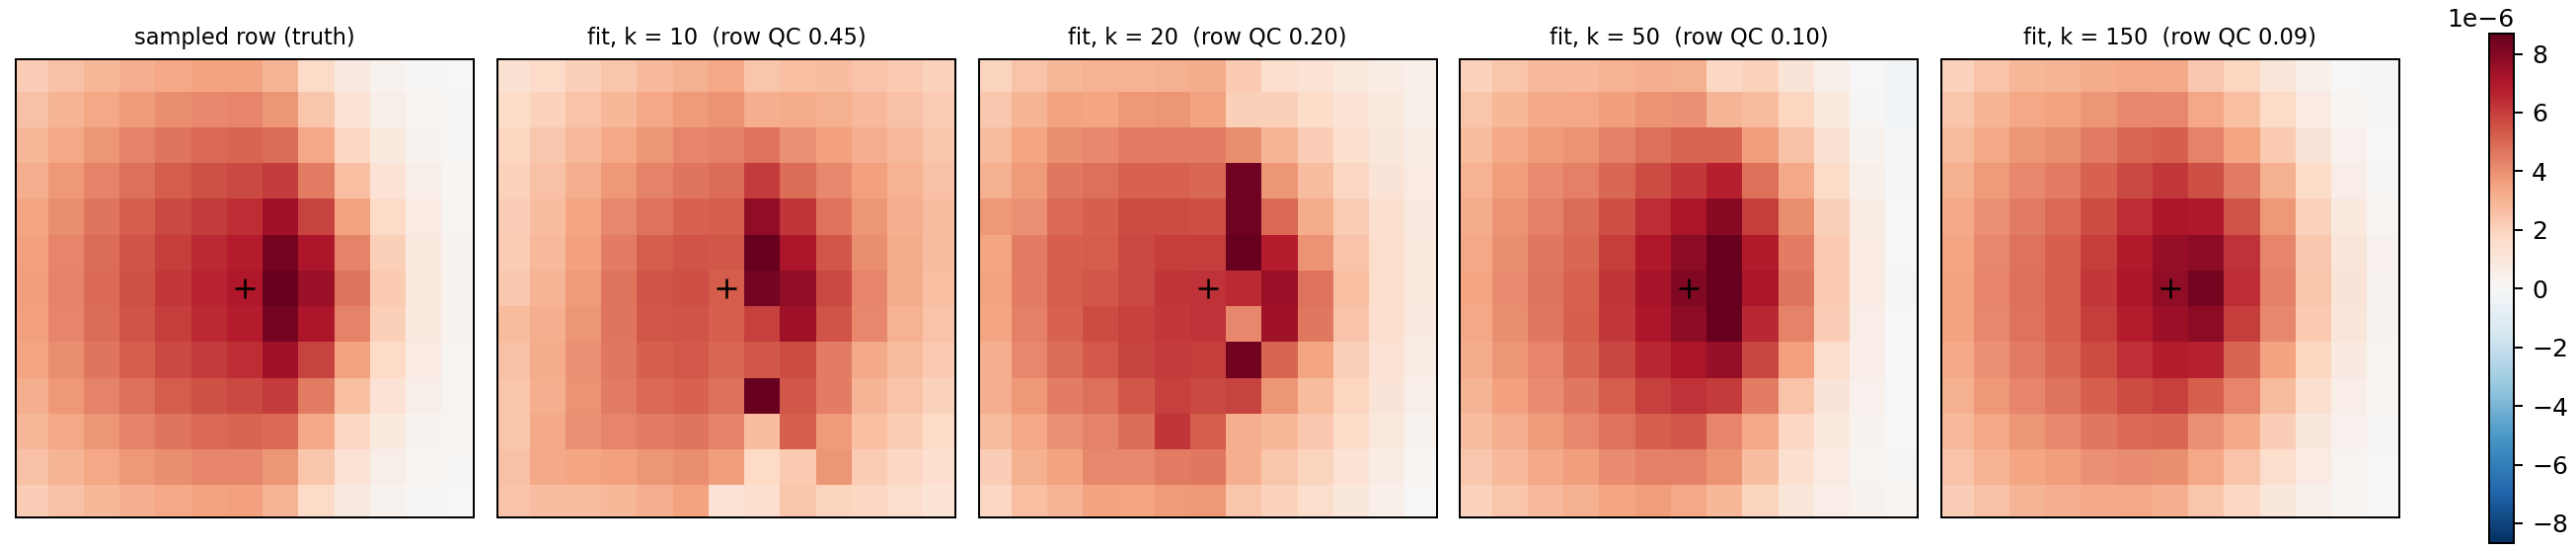
\includegraphics[width=\textwidth]{figures/psf_fit.png}
  \caption{\textbf{(One row, fitted.)} The slab-side interface row of
    Figure~\ref{fig:psfs}(b)'s type, chosen so its held-out scores track
    the interface-region median at every budget --- a representative
    hard row, not a best case. All five panels share one color scale.
    At $k = 10$ the fit is blotchy; at $k = 20$ the shape is right but
    an artifact ridge stands at the interface; by $k = 50$ the row is
    essentially correct; $k = 150$ is a close match. Titles give each
    fit's held-out score for this row.}
  \label{fig:fit}
\end{figure}

\section{Certify, then price: the corrections build}
\label{sec:build}

The assembled $B$ is an \emph{estimate} of $\Hd$, and estimates carry
noise: the fit error puts spurious negative modes into the pencil
$(B, \Hr)$ --- 345 of them here. A preconditioner built from $B + a\Hr$
must be certified positive definite before conjugate gradients may
trust it. \texttt{make\_pd} runs Lanczos sweeps in the $\Hr$ inner
product, flips the pencil modes below the build threshold (only 3 of
the 345 matter at build shift $a_0 = 10^{-5}$), and certifies a
\emph{floor}: the corrected operator $B + E + a\Hr$ is provably
positive definite for every $a$ above $-\lambda_{\mathrm{floor}} =
3.7\times 10^{-6}$. The flips cost $\Hr$-solves --- no PDE solves. A
\emph{value pass} then spends a small budget of true Hessian
applications (here 30) measuring and correcting the largest remaining
fit errors:

{\small\begin{verbatim}
# One certified operator struct from the fit and its probe archive.
# make_pd flips the few pencil modes below the build threshold (an
# Hr-solve currency -- no PDE solves) and certifies a floor: the
# shifts a at which B + E + a Hr is provably positive definite. The
# value pass then spends a small budget of TRUE Hessian applies
# pricing the error the fit left behind.
archive = corr.ProbeArchive()
archive.Z, archive.Y = V.T.copy(), HV.T.copy()
A = corr.make_shifted_operator(corr.sparse_op(B), archive,
                               corr.sparse_hr_oracle(problem["Hr"]), A0)
report = corr.make_pd(A, max_iters=3000)
assert report.certified
Hd_op = corr.SymmetricOp(problem["count"], problem["apply_Hd"])
corr.value_pass(A, Hd_op, VP_APPLIES, corr.ValuePassMode.V2)
\end{verbatim}
}

Every later solve is checked against these contracts: shifts at or
above $a_0$ are guaranteed, shifts between the floor and $a_0$ proceed
with a runtime certificate, and shifts at or below the floor are
refused --- not timidity; the operator is provably indefinite there.
The formulas behind the layer are documented in
\texttt{dev/pencil-corrections-notes.pdf} in the lgpsf repository.

\section{One build, every shift: the L-curve}
\label{sec:lcurve}

Choosing the regularization parameter means solving the normal
equations at many shifts. The build above serves all of them: changing
$a$ is scalar arithmetic, with nothing refactored. Each solve is outer
PCG on the \emph{true} operator --- one PDE-based Hessian application
per iteration --- with the corrected struct as the preconditioner:

{\small\begin{verbatim}
# The whole sweep runs on the one build: changing the shift is scalar
# arithmetic, zero refactorization. Each solve is outer PCG on the
# TRUE operator (one PDE-based Hessian apply per iteration) with the
# corrected struct as the preconditioner. When the diagnostic tail
# crosses below the certified floor the solve is REFUSED, and
# rebuild_at re-anchors every contract from the archive: new flips
# cost Hr-solves only, and the value-pass pairs refold in exactly,
# with zero new PDE solves.
for a in SWEEP:
    if corr.classify_shift(A, a).zone == corr.Zone.Refused:
        report = corr.rebuild_at(A, SWEEP.min(), max_iters=3000)
    u, iterations = solve_at(a)
    record(a, u, iterations)
\end{verbatim}
}

We sweep eleven shifts from $10^{-2}$ down to $10^{-7}$
(Figure~\ref{fig:lcurve}). The solves cost 5 PCG iterations at
$a = 10^{-2}$, growing to 16 at the build shift. The sweep's diagnostic
tail then crosses the certified floor, the solve is refused, and
\texttt{rebuild\_at} re-anchors the contracts at the smallest shift in
the sweep: 144 newly windowed modes flip ($\Hr$-solve work only), the
archived value-pass pairs fold back in exactly by linearity, and the
tail proceeds --- 22 to 150 iterations, the honest price of the
under-regularized regime, where the true system's conditioning is
brutal for any method. The discrepancy principle
($\|A u_0 - d\| = \sigma\sqrt{n}$, with the noise level $\sigma$ known
here by construction) picks $a^\ast = 1.3\times 10^{-5}$, squarely at
the corner.

\begin{figure}[htb]
  \centering
  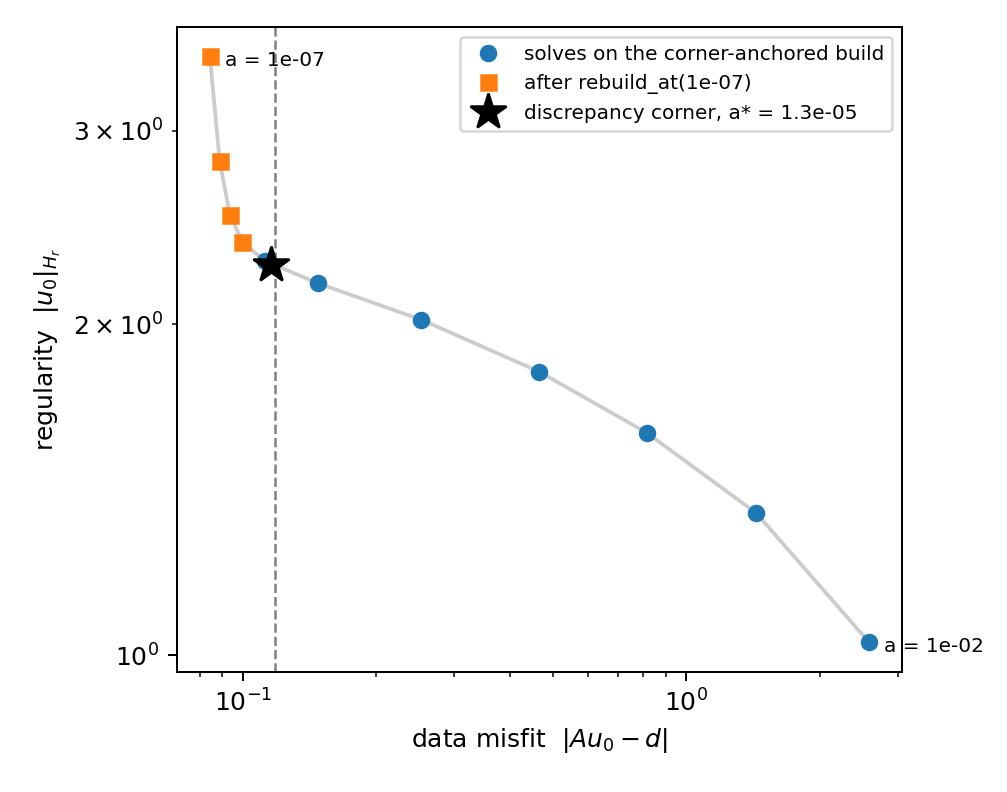
\includegraphics[width=0.62\textwidth]{figures/lcurve.png}
  \caption{\textbf{(The L-curve, one build.)} Data misfit against
    regularity for eleven shifts spanning five decades. Blue circles:
    solves on the corner-anchored build. Orange squares: the diagnostic
    tail, served by the same archive after \texttt{rebuild\_at} ---
    zero new PDE solves. The star marks the discrepancy corner
    $a^\ast = 1.3\times 10^{-5}$; the dashed line is the discrepancy
    level $\sigma\sqrt{n}$.}
  \label{fig:lcurve}
\end{figure}

Figure~\ref{fig:recon} shows reconstructions at three shifts. The
corner reconstruction recovers everything the data still contains ---
the blob, the background spot, the pocket spot --- and does not recover
the slab spots, which Figure~\ref{fig:problem} showed were smeared away
before the data was ever recorded. Too little regularization buys
noise, not slab spots.

\begin{figure}[htb]
  \centering
  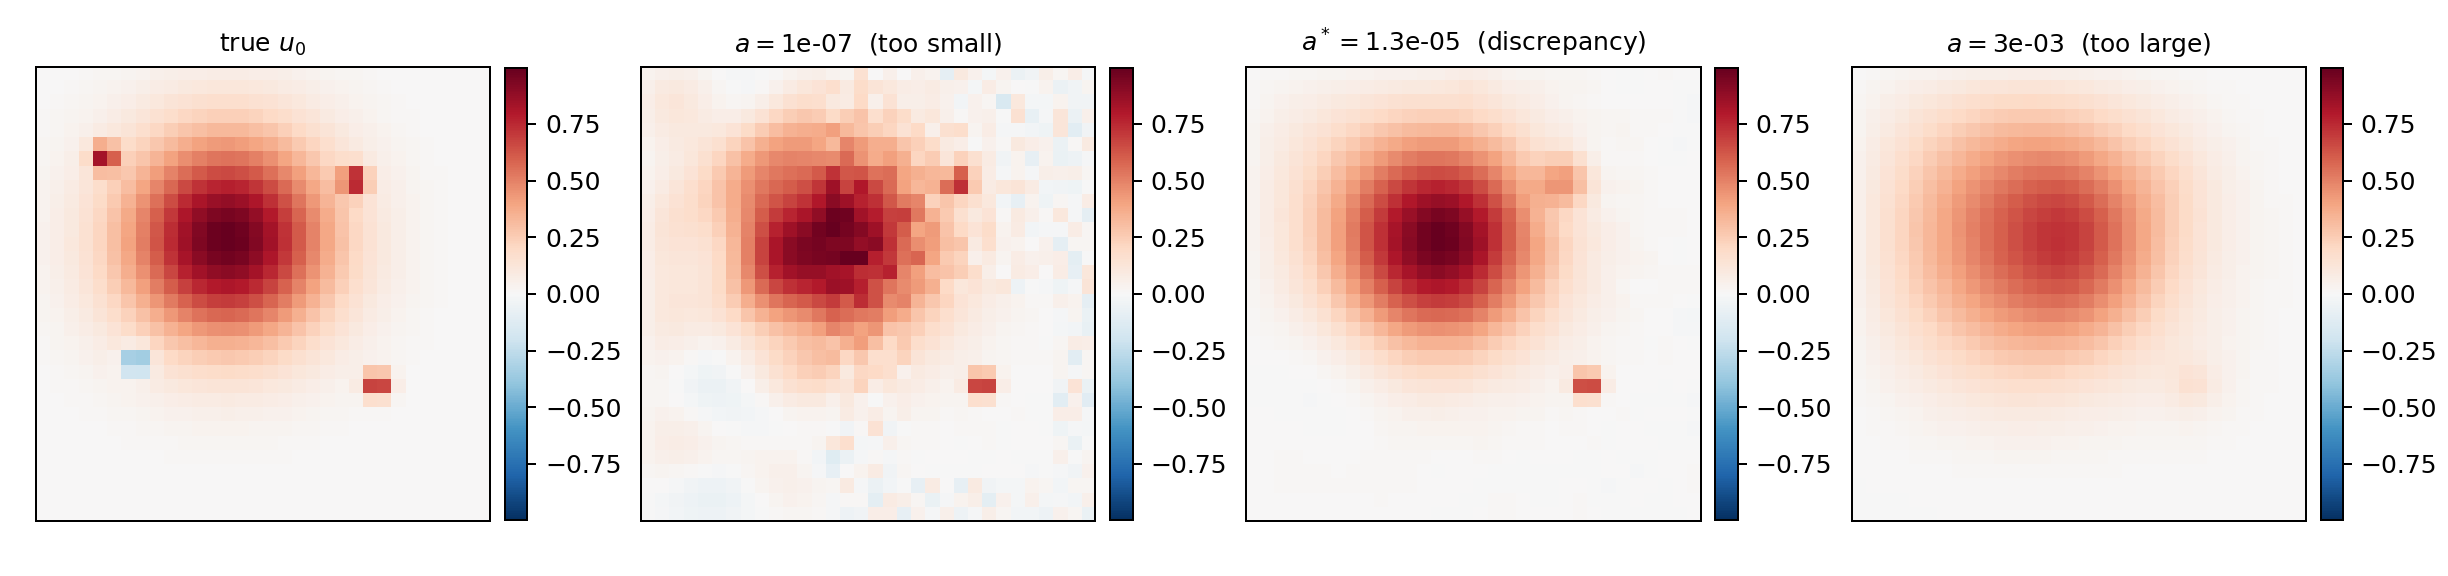
\includegraphics[width=\textwidth]{figures/recon.png}
  \caption{\textbf{(Reconstructions.)} Truth, then three shifts from
    the sweep, one color scale. At $a = 10^{-7}$ the reconstruction
    overfits noise; at the discrepancy corner it recovers exactly the
    features the data retains; at $a = 3\times 10^{-3}$ the blob
    survives but every spot is smoothed away.}
  \label{fig:recon}
\end{figure}

\section{What the build buys: spectra, iterations, cost}
\label{sec:spectra}

All results in this section are at the corner $a^\ast$. The quantity
that governs PCG is the preconditioned spectrum; flat at 1 is the goal.
Figure~\ref{fig:spectra} shows it three ways.

\textbf{(a) The probe budget.} Regularization-only preconditioning ---
the standard fallback, spectrum $1 + \lambda_i/a^\ast$ --- spans
$3.7\times 10^{3}$. The certified fits compress that to $15.1$, $6.4$,
$3.5$, $3.1$ at $k = 10, 20, 50, 150$: two orders of magnitude from ten
probes, then diminishing returns, because the surviving tail comes from
the hard interface rows rather than from resolution the next probe
could buy.

\textbf{(b) The symmetrization.} lgpsf fits rows independently, so the
raw assembly is nonsymmetric and admits no certificate (its spectrum
here is the singular values of the one-sided preconditioned operator;
for comparability all three curves in the panel are computed that way
--- for the two symmetric variants these tell the same story as the
eigenvalues, to which they agree up to symmetric similarity, not
entry-for-entry). As fitted: condition $9.6$. Plain averaging: $7.6$
--- averaging lets a strong row's tail contaminate its weak neighbor.
The weighted symmetrization, which trusts each entry's better-resolved
row: $3.5$. Symmetry is not bookkeeping; it is worth a factor of three
here.

\textbf{(c) The deflation.} At this lean budget, \emph{free} deflation
--- re-using the fit probes' residuals at no extra cost --- makes the
tail \emph{worse} (condition 15): with only 50 probes the residual
basis is too noisy to point at true error directions, and we show this
rather than hide it. The value pass is the resolution: 30 true
applications, spent measuring rather than guessing, tamp the tail and
give the best operator in this document (condition $2.45$).

\begin{figure}[htb]
  \centering
  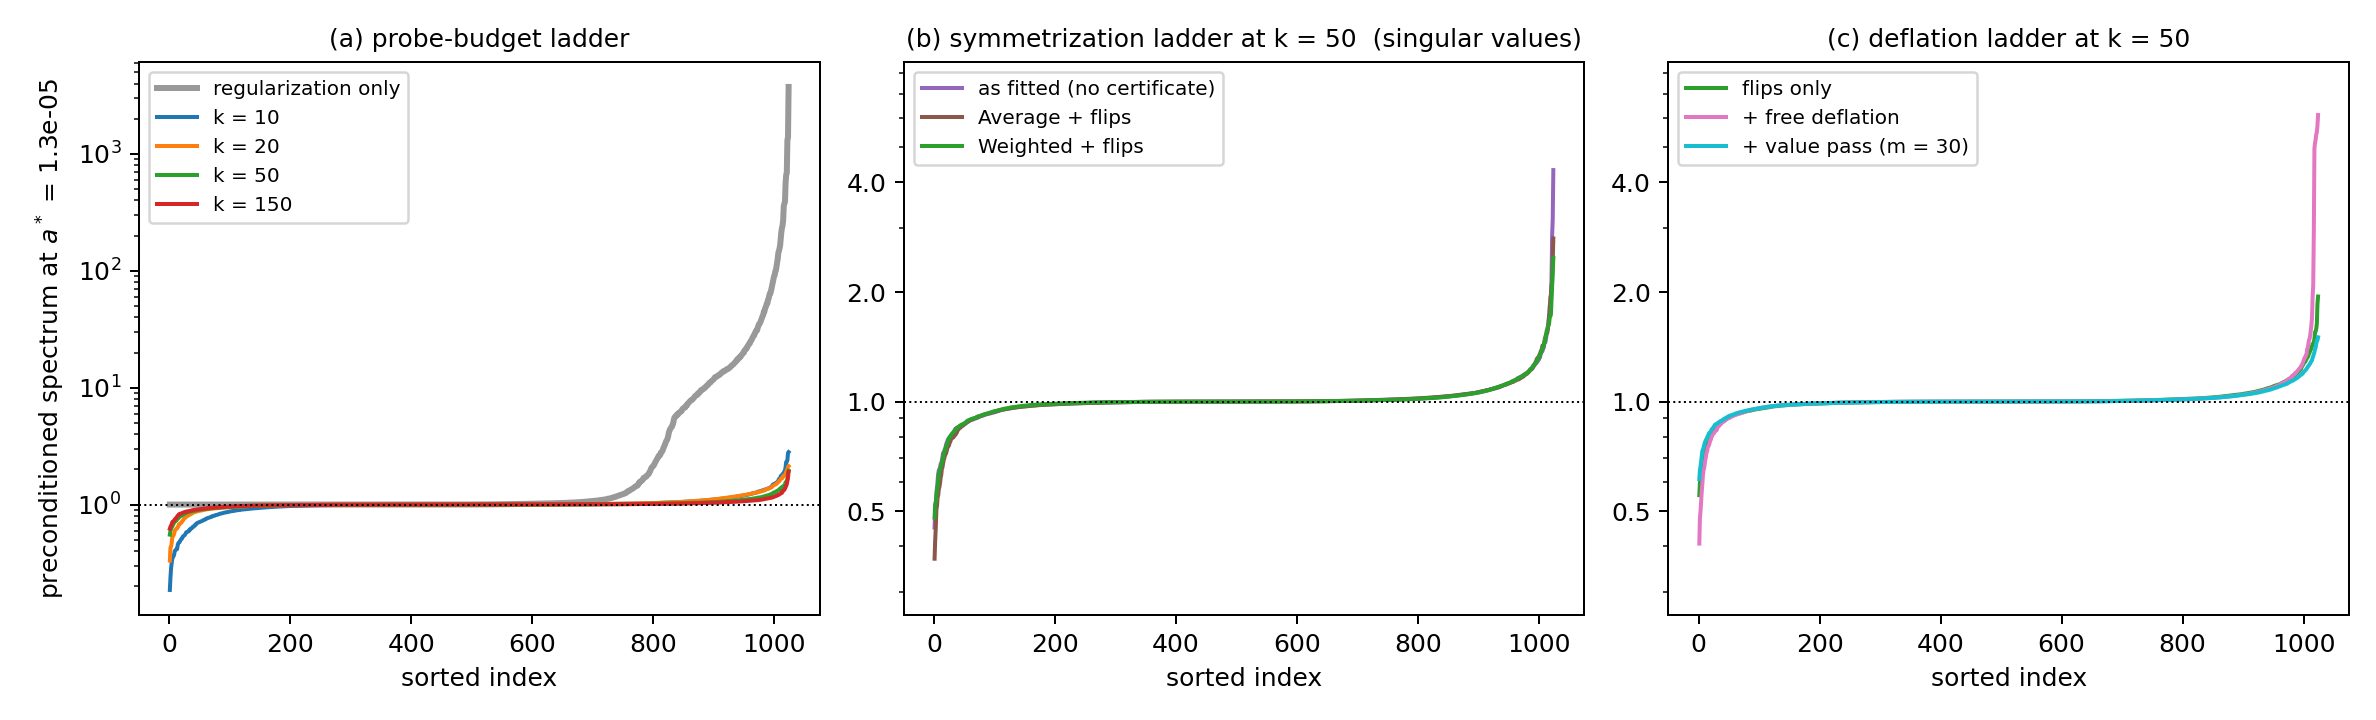
\includegraphics[width=\textwidth]{figures/spectra.png}
  \caption{\textbf{(Preconditioned spectra at $a^\ast$.)} Sorted
    spectrum of the preconditioned system, one curve per variant;
    dotted line at 1. (a) Regularization-only against the certified
    weighted fits at four budgets --- note the vertical scale.
    (b) The symmetrization ladder at $k = 50$, all three curves as
    one-sided preconditioned singular values; panels (b) and (c) share
    a vertical scale far tighter than (a)'s. (c) The deflation ladder at
    $k = 50$: free deflation spikes the tail; the 30-apply value pass
    tamps it below the flips-only curve.}
  \label{fig:spectra}
\end{figure}

The convergence curves (Figure~\ref{fig:convergence}) are the spectra
made kinetic: 166 iterations under regularization preconditioning
against 32, 17, 15 for the fitted budgets and 14 for the value-passed
build --- each iteration one PDE-based Hessian application. The cost ledger, counting
every application of $\Hd$ each preconditioner consumed:

\begin{center}
\begin{tabular}{l r r}
\hline
preconditioner & probes & condition number \\
\hline
regularization only & 0 & 3745 \\
Weighted + flips, k = 10 & 10 & 15.1 \\
Weighted + flips, k = 20 & 20 & 6.43 \\
Weighted + flips, k = 50 & 50 & 3.51 \\
Weighted + flips, k = 150 & 150 & 3.07 \\
k = 50 + free deflation & 50 & 15 \\
k = 50 + value pass (m = 30) & 80 & 2.45 \\
as fitted, k = 50 (sing. values) & 50 & 9.59 \\
Average + flips, k = 50 (sing. values) & 50 & 7.58 \\
\hline
\end{tabular}

\end{center}

\noindent
Read the middle column against the right one. Fifty probes plus thirty
priced applications buy a condition number of $2.45$; the same eighty
applications spent as bare PCG iterations under regularization
preconditioning would not even reach the discrepancy tolerance once.

\begin{figure}[htb]
  \centering
  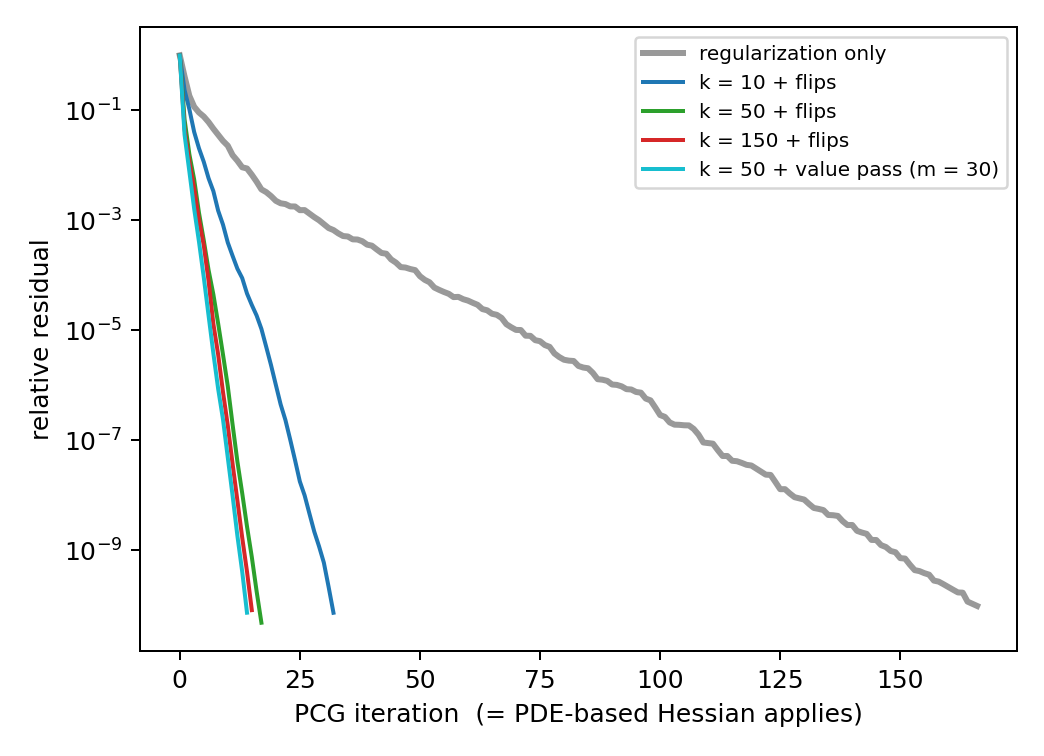
\includegraphics[width=0.62\textwidth]{figures/convergence.png}
  \caption{\textbf{(PCG convergence at $a^\ast$.)} Relative residual
    against iteration for the variants of
    Figure~\ref{fig:spectra}(a,c). The ordering, spacing, and
    near-straight slopes are exactly what the spectra promise.}
  \label{fig:convergence}
\end{figure}

\section{All scales at once}

Why does the fitted preconditioner matter beyond iteration counts?
Because of \emph{which} components arrive first.
Regularization-preconditioned CG builds the solution coarse-to-fine:
smooth components converge quickly and fine-scale features arrive last,
so the weak background spot only materializes between iterations 16 and
40 (Figure~\ref{fig:iterates}, top). The lgpsf-preconditioned iteration
whitens all scales at once: its first iterate is rough --- blob, spots,
and fine-scale content all present immediately --- and by iteration 5
it is converged. If the iteration must be truncated early, the two
preconditioners do not merely differ in speed; they return different
kinds of partial answers.

\begin{figure}[htb]
  \centering
  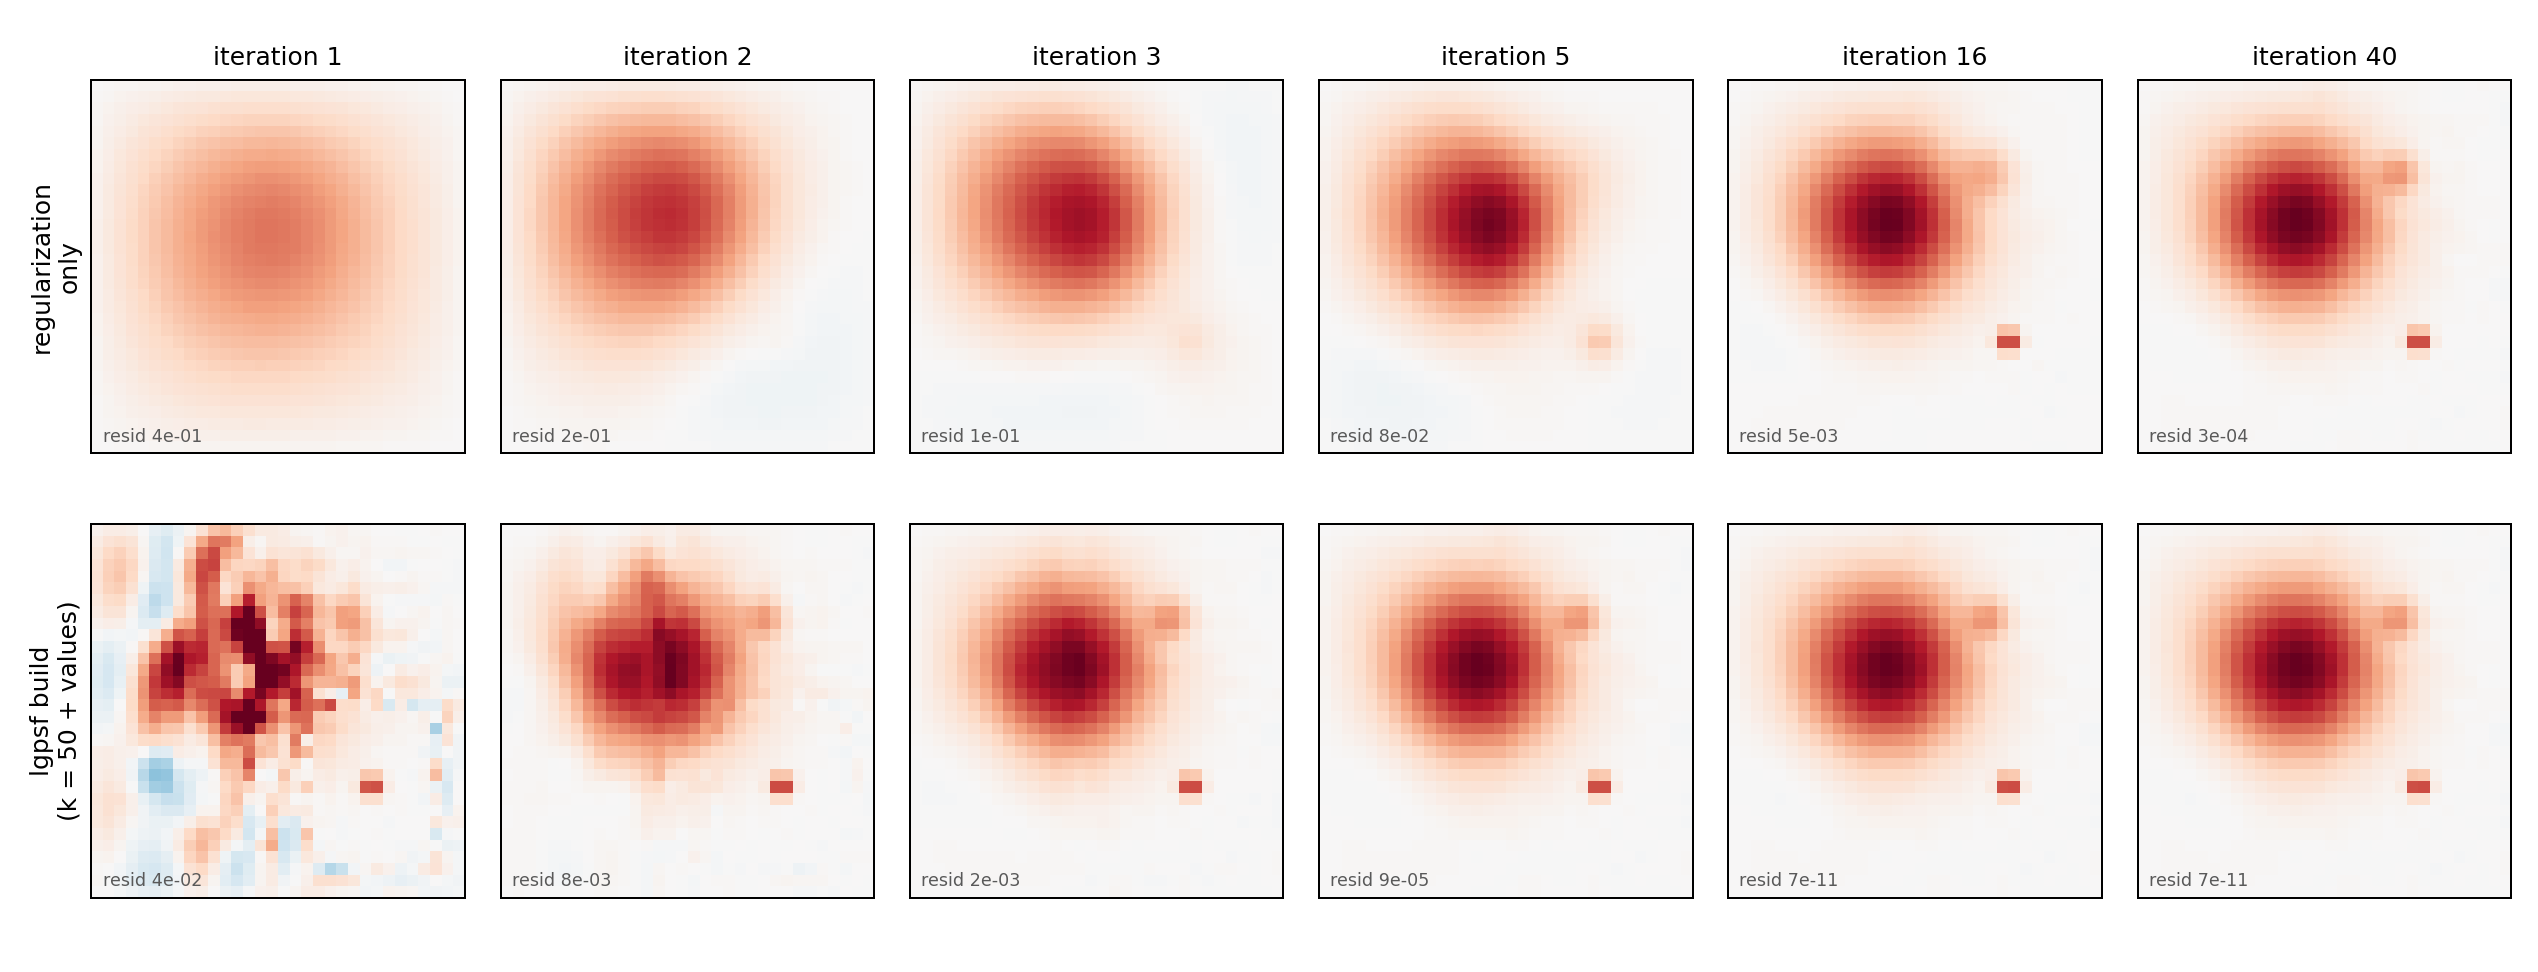
\includegraphics[width=\textwidth]{figures/iterates.png}
  \caption{\textbf{(PCG iterates as images.)} Reconstruction iterates
    at matched iterations, one color scale; each panel is annotated
    with its run's relative residual. Top row: regularization-only ---
    the blob first, the pocket spot by iteration 5, the weak background
    spot only between 16 and 40. Bottom row: the lgpsf build --- every
    scale present from iteration 1, converged by 5.}
  \label{fig:iterates}
\end{figure}

\section{Reproducing this document}

\texttt{docs/heat-pipeline/make\_figures.py} produces every figure,
number, and snippet above from scratch (\texttt{--items} selects
stages; intermediate results are cached under \texttt{cache/}, and
deleting that directory forces full regeneration --- under an hour on
a laptop, nearly all of it in the regularization sweep and the
certified builds). The problem definition lives in
\texttt{examples/}, module \texttt{heat\_inversion.py}; the four worked
examples there teach the same corrections API one lesson at a time.
Constants: grid $32$, noise $1.5\%$, data seed $20260803$, fit probes
from seed $0$, held-out probes from seed $101$.

\end{document}
